\chapter{Implementacja}

W niniejszym rozdziale przedstawiono szczegóły techniczne zaimplementowanego rozwiązania. Omówione zostaną kluczowe aspekty
implementacyjne systemu, obejmujące wykorzystanie platformy Microsoft Power Platform - w szczególności
Power Apps do budowy interfejsu użytkownika oraz Power Automate do automatyzacji procesów biznesowych.
Ponadto, przedstawiona zostanie integracja z platformą SharePoint oraz implementacja skryptów
usprawniających pracę z pakietem Microsoft Office. Rozdział stanowi techniczne rozwinięcie przyjętych
założeń projektowych, prezentując metodykę realizacji poszczególnych komponentów systemu.

W ramach analizy technicznej zostaną szczegółowo omówione poszczególne komponenty systemu oraz sposób
ich integracji. Szczególna uwaga zostanie poświęcona mechanizmom przepływu danych, automatyzacji
procesów oraz implementacji logiki biznesowej w środowisku low-code. Istotnym elementem będzie również
prezentacja zastosowanych rozwiązań w zakresie bezpieczeństwa danych oraz optymalizacji wydajności
w kontekście platformy Microsoft 365.

\section{Ekran zapisu danych}

Zdecydowano, że pierwszym ekranem aplikacji będzie ekran zapisu danych. Decyzja ta wynika z faktu, że bez prztworzonych danych, utworzenie innych ekranów byłoby zdecydowanie trudniejsze. Ekran ten składa się z elementów, które zostaną omówione poniżej.

\subsection{Zapis pliku w chmurze}
Pierwszym krokiem jest zapis pliku w chmurze w celu udostepnienia go innym systemom. W tym celu wykorzystano kontrolkę\footnote{Kontrolka -- element służący do nawigacji, wyświetlania danych i obsługi aplikacji.} \emph{Attachment Control}. Pozwala ona na zapisanie pliku w pamięci aplikacji. Odbywa się to przez naciśnięcie przycisku \emph{"Dołącz plik"} lub przy użyciu mechaniki \emph{przeciągnij i upuść} (\english{Drag And Drop}). 

Aby przekazać plik oraz jego zawartość należy nacisnąć przycisk opisany jako \emph{Save attachments} znajdujący się pod wcześniej omawianym elementem. Naciścięcie go skutkuje wywołaniem szeregu funkcji opisanych we właściwości \emph{OnSelect}. W pierwszej kolejności sprawdzane jest, czy plik został załadowany. Jeśli tak, to wywoływany jest przepływ \emph{SaveFileAndRunScript}. Wynik przepływu jest zapisywany w zmiennej tablicowej, która w Power Apps określana jest jako \definicja{kolekcja}, o nazwie \emph{FlowOutput}. Po wykonaniu się przepływu, zapisane w kontrolce pliki są usuwane.

\subsubsection{Przepływ SaveFileAndRunScript}
Przepływ \emph{SaveFileAndRunScript} jest odpowiedzialny za zapisanie pliku w chmurze. W momencie wywołania przepływu plik jest przekazany jako parametr wejściowy. Przepływ ten składa się z kilku kroków, które zostaną omówione w kolejności ich wykonywania.

\begin{figure}[H]
    \centering
    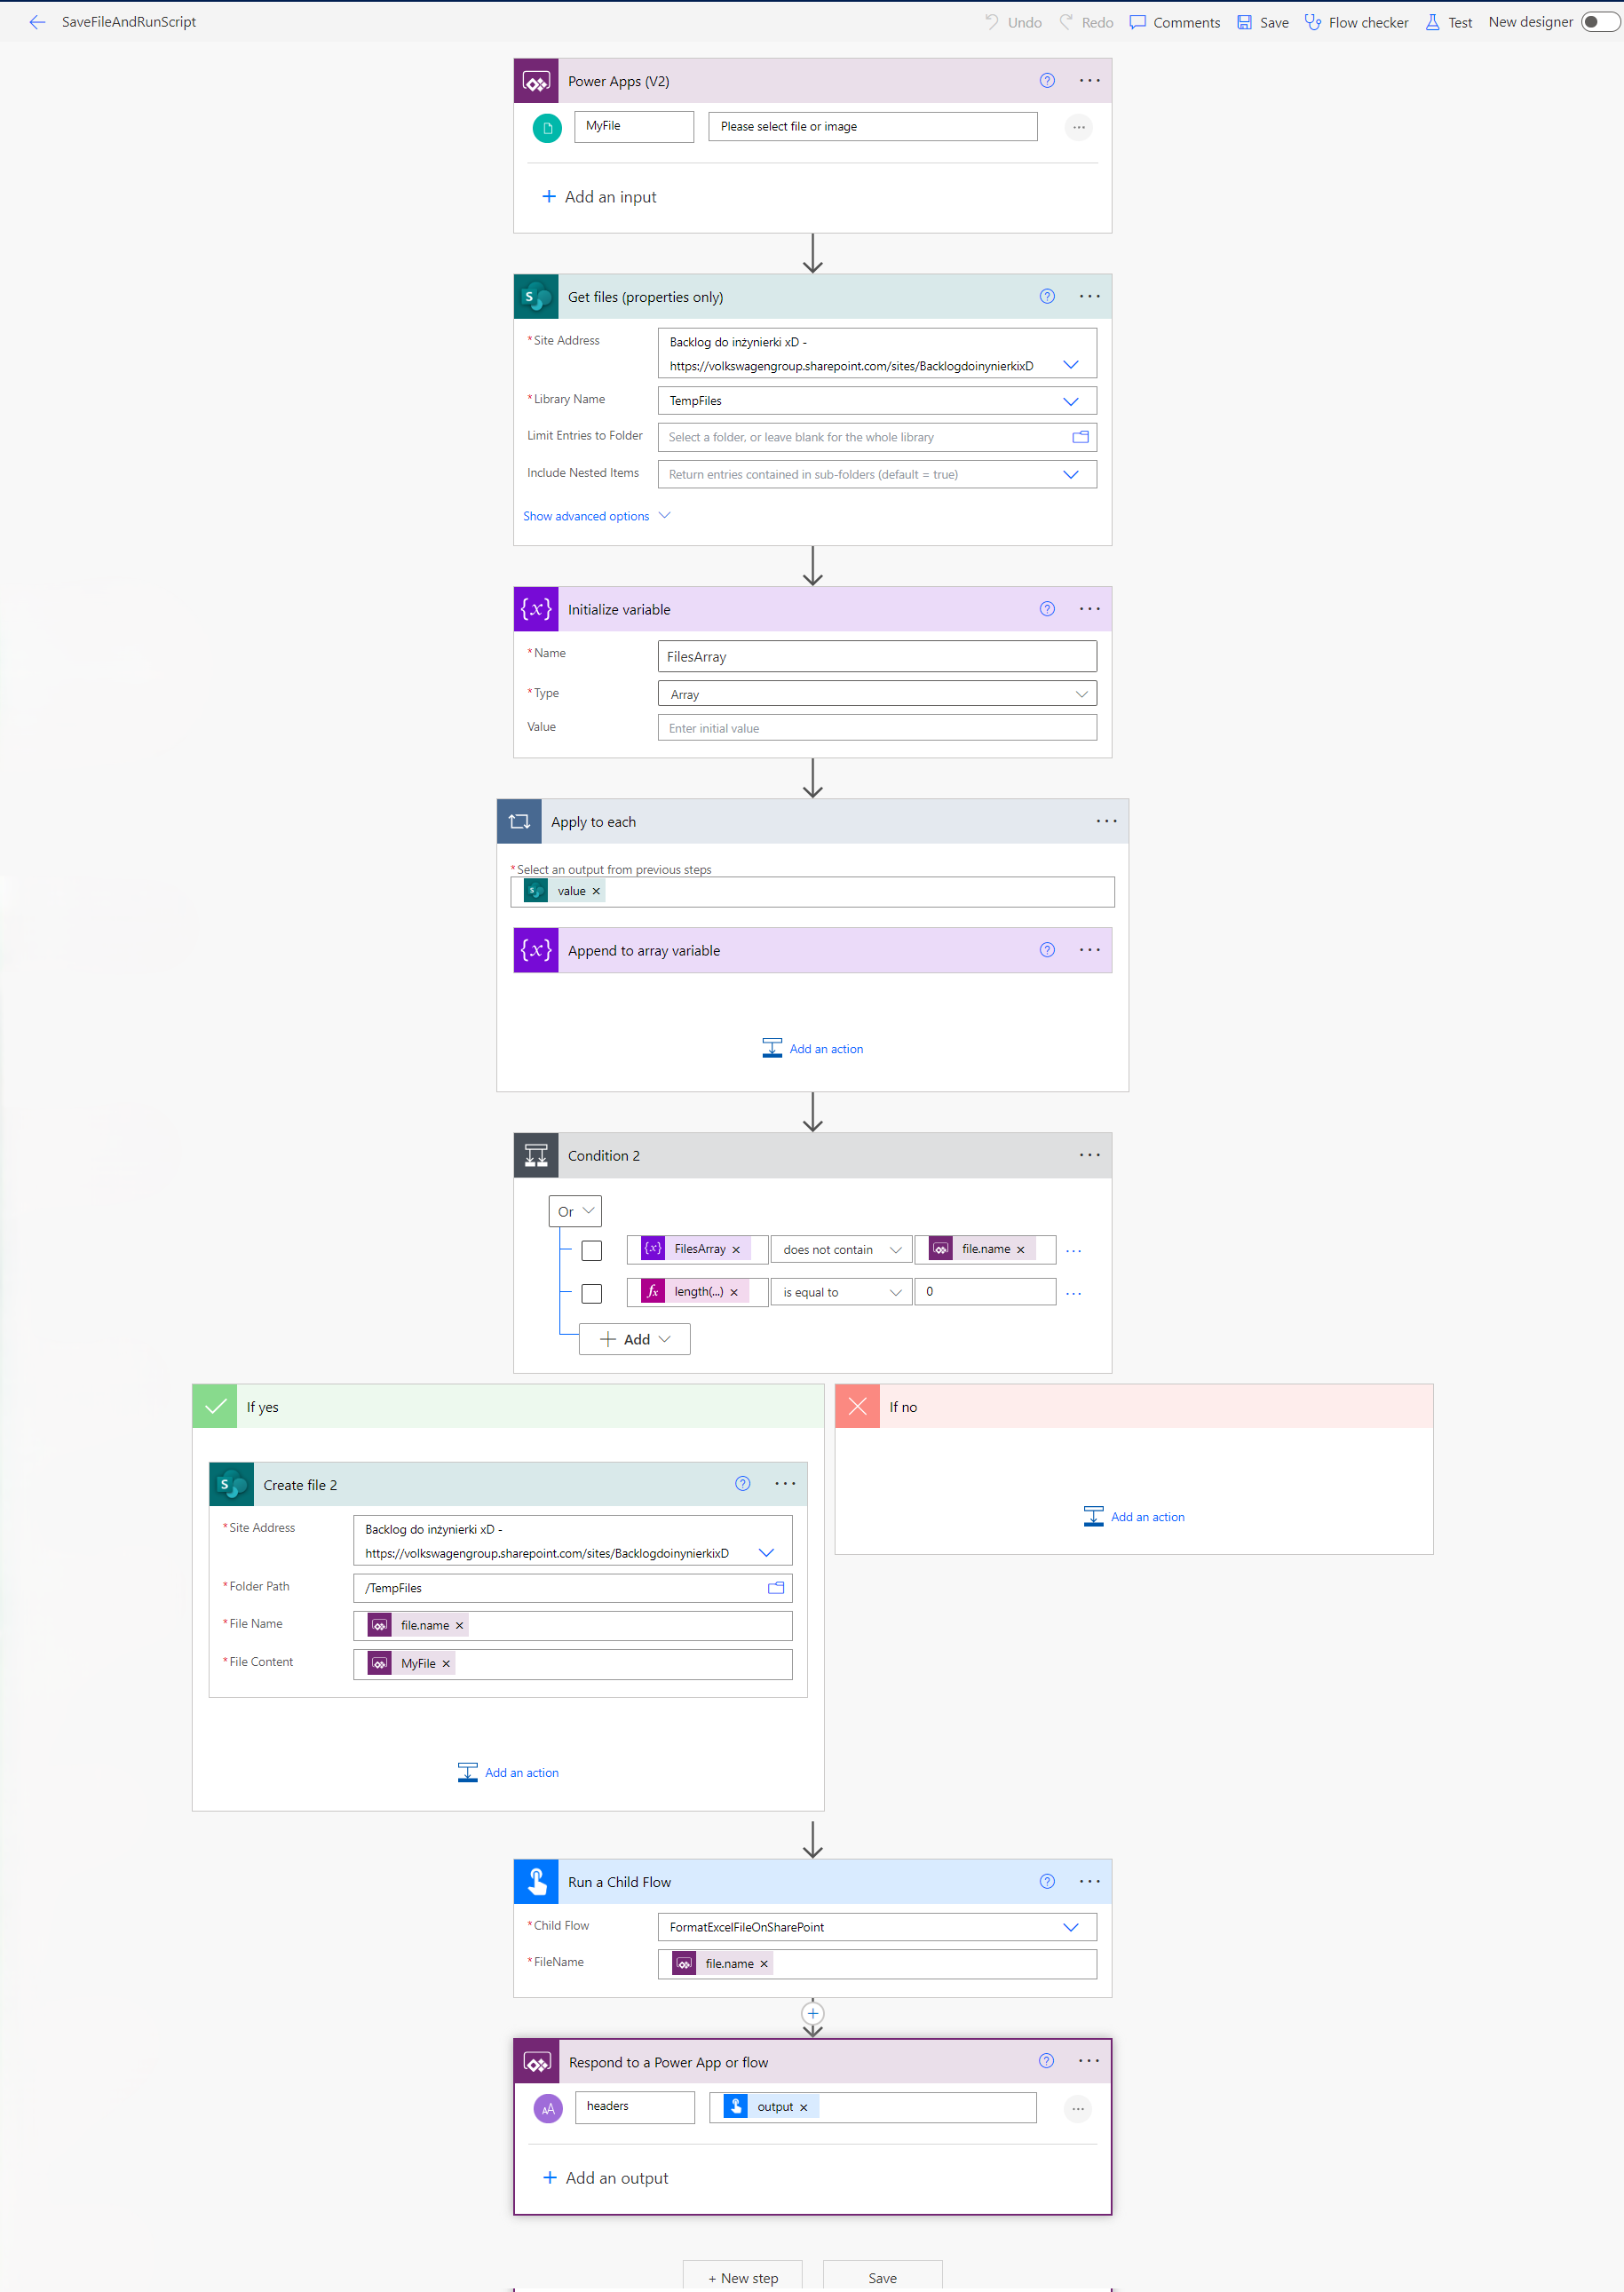
\includegraphics[width=0.85\textwidth]{figures/SaveFileAndRunScript.png}
    \caption{Widok przepływu SaveFileAndRunScript}
    \label{fig:savefileandrunscript}
\end{figure}

Rysunek \ref{fig:savefileandrunscript}, przedstawia widok przepływu \emph{SaveFileAndRunScript}. Przepływ ten składa się z następujących kroków:
\begin{enumerate}
    \item \textbf{Funkcja: Power Apps (V2)} \\
    Jest to element rozpoczynający przepływ, wywoływany bezpośrednio z aplikacji Power Apps. Parametrami wejściowymi są:
    \begin{itemize}
        \item nazwa pliku (\textit{File Name}),
        \item zawartość pliku (\textit{File Content}) w formacie binarnym.
    \end{itemize}

    \item \textbf{Sprawdzenie istniejących plików} \\
    Blok \textit{Get files (properties only)} pobiera listę wszystkich plików z wybranego folderu SharePoint wraz z ich metadanymi, takimi jak nazwa, ścieżka czy data modyfikacji. Pozwala to na sprawdzenie, czy plik o podanej nazwie już istnieje w bibliotece.

    \item \textbf{Warunek} \\
    Element \textit{Condition} sprawdza, czy istnieje plik o nazwie przekazanej w danych wejściowych. W zależności od wyniku:
    \begin{itemize}
        \item jeśli plik istnieje -- przepływ kończy działanie,
        \item jeśli plik nie istnieje -- kontynuuje proces zapisu.
    \end{itemize}

    \item \textbf{Utworzenie pliku} \\
    Blok \textit{Create file} tworzy nowy plik w SharePoint, wykorzystując parametry:
    \begin{itemize}
        \item adres witryny SharePoint,
        \item ścieżkę do folderu docelowego,
        \item nazwę pliku,
        \item zawartość pliku.
    \end{itemize}

    \item \textbf{Uruchomienie podprzepływu} \\
    Element \textit{Run a Child Flow} wywołuje skrypt Office Script, który:
    \begin{itemize}
        \item analizuje zapisany plik,
        \item sprawdza jego zawartość,
        \item formatuje dane według wymagań,
        \item zwraca wynik w formacie JSON.
    \end{itemize}

    \item \textbf{Odpowiedź do aplikacji} \\
    Blok \textit{Respond to Power Apps} kończy przepływ, zwracając do aplikacji dane w formacie JSON przetworzone przez wcześniej wspomniany skrypt Office Script.
\end{enumerate}

\subsection{Skrypt Office Script}
Po utworzeniu pliku w SharePoint, w ramach przepływu następuje jego przetworzenie przez skrypt Office Script. W tym przypadku skrypt ma za zadanie przeanalizować plik i dostosować go do wymagań systemu. Poniżej przedstawiono kroki działania skryptu:

\begin{enumerate}
    \item \textbf{Inicjalizacja i wybór arkusza}
    \begin{itemize}
        \item sprawdzenie wszystkich arkuszy w pliku Excel,
        \item wybór arkusza zawierającego dane,
        \item sprawdzenie i ewentualne usunięcie ochrony hasłem.
    \end{itemize}

    \item \textbf{Analiza danych}
    \begin{itemize}
        \item sprawdzenie czy dane są zorganizowane w tabeli,
        \item w przypadku braku tabeli -- utworzenie nowej,
        \item automatyczne uzupełnienie pustych miejsc w ważnych kolumnach.
    \end{itemize}

    \item \textbf{Dopasowanie nazw kolumn}
    \begin{itemize}
        \item porównanie istniejących nazw kolumn ze standardową listą,
        \item wykorzystanie algorytmu \emph{Jaro-Winkler} do oceny podobieństwa tekstu,
        \item automatyczne rozpoznawanie podobnych nazw (np. "Srv ID" jako "Service ID"),
        \item sugestia ręcznego wyboru przy zbyt małym podobieństwie (poniżej 90\%).
    \end{itemize}

    \item \textbf{Przekazanie wyników}
    \begin{itemize}
        \item zwrócenie oryginalnych nazw kolumn z pliku,
        \item zwrócenie dopasowanych standardowych nazw kolumn,
        \item w razie problemów - przekazanie odpowiednich komunikatów błędów.
    \end{itemize}
\end{enumerate}


\vspace{1cm}
Po zakończeniu działania skryptu Office Script i całego przepływu, przetworzony plik zostaje w pełni zapisany w bibliotece SharePoint. 
Rysunek \ref{fig:saveattachmentsform} przedstawia wspomnianą wcześniej kontrolkę \emph{Attachment Control}, przycisk \emph{Save attachments} oraz listę plików zapisanych w foldrze SharePoint.


\begin{figure}[h]
    \centering
    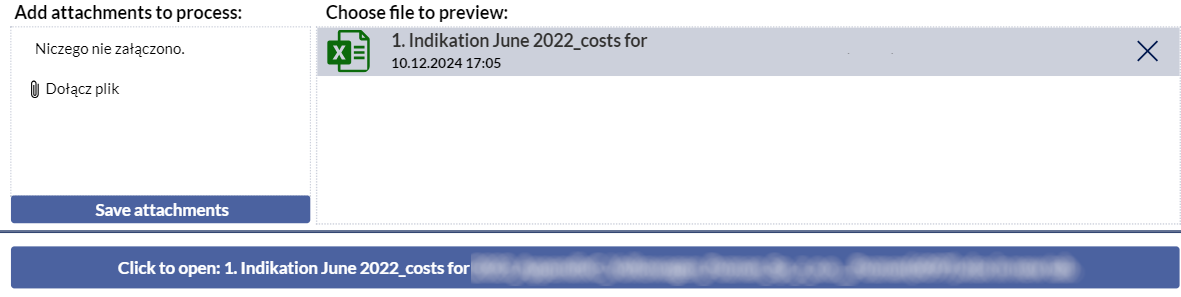
\includegraphics[width=\textwidth]
    {figures/SaveAttachmentsForm.png}
    \caption{Formularz zapisu pliku}    
    \label{fig:saveattachmentsform}
\end{figure}

Wybór elementu z listy \emph{Choose file to preview} umożliwia wskazanie pliku do dalszego przetwarzania. Selekcja pozycji z listy automatycznie inicjuje wykonanie opisanego wcześniej skryptu, którego celem jest pozyskanie aktualnego zestawu nagłówków. Należy podkreślić, że ten sam proces zachodzi również podczas inicjalizacji aplikacji. 
Funkcjonalność podglądu, zaimplementowana w postaci przycisku umiejscowionego poniżej głównych elementów sterujących, umożliwia otwarcie wybranego pliku w nowej karcie przeglądarki. Jest to szczególnie istotne w kontekście weryfikacji poprawności danych oraz walidacji struktury kolumn.